\documentclass[10pt,draftclsnofoot,onecolumn]{IEEEtran}
\hyphenation{op-tical net-works semi-conduc-tor}

\usepackage[margin=.75in]{geometry}
\usepackage{courier}
\usepackage{ifthen}
\usepackage{setspace}
\usepackage{listings}
\usepackage[usenames, dvipsnames]{color}
\usepackage{tabularx}
\usepackage[strict]{chngpage}
\usepackage{cite}
\usepackage{graphicx}
\usepackage{acronym}
\usepackage{color}
\usepackage{makeidx}
\usepackage{url}
\usepackage{listings}
\usepackage{verbatim}

\makeindex

\acrodef{NPM}[NPM]{Node Package Manager}
\acrodef{OSU}[OSU]{Oregon State University}
\acrodef{AIAA}[AIAA]{American Institute of Aeronautics and Astronautics}
\acrodef{COCOM}[COCOM]{Coordinating Committee for Multilateral Export Controls}

\lstset {
	language=C,
	basicstyle=\ttfamily,
	keywordstyle=\color{blue}\ttfamily,
	stringstyle=\color{red}\ttfamily,
	commentstyle=\color{OliveGreen}\ttfamily,
	morecomment=[l][\color{magenta}]{\#}
	showstringspaces=false,
	showspaces=false,
	frame=single,
	captionpos=b
}

\newcommand{\commandline}[2][\empty] {
	\begin{quote}
		\texttt{#2}
		\ifthenelse{\equal{#1}{\empty}}{}{\begin{quote}#1\end{quote}}
	\end{quote}
}

\newcommand{\sigline}[1][\empty] {
	\vspace{1in}
	\hrule width0.5\textwidth
	\vspace{1mm}
	\noindent #1	
}

\newcommand*{\SignatureAndDate}[1]{
	\vspace{1in}
	\par\noindent\makebox[2.5in]{\hrulefill} \hspace{.5in} \makebox[2.0in]{\hrulefill}
	\par\noindent\makebox[2.5in][l]{#1}      \hspace{.5in} \makebox[2.0in][l]{Date}
}

\newcommand{\newentity}[5]{

	\noindent\textbf{#2}
	
	\noindent Entity
	
	\noindent\textit{Author:} {#1}
		
	\noindent\textit{Type:} {#3}
	
	\noindent\textit{Purpose:} {#4}

	\noindent\textit{Contents:} {#5}
	\vspace{.5cm}

}


\newcommand{\newinterface}[5]{

		\noindent\textbf{#2}
		
		\noindent Entity
		
		\noindent\textit{Author:} {#1}
		
		\noindent\textit{Function:} {#3}
		
		\noindent\textit{Interface:} {#4}		

		\noindent\textit{Contents:} {#5}
		\vspace{.5cm}
}


\newcommand{\newrelationship}[4]{
	\noindent\textbf{#2}
	
	\noindent Relationship
	
	\noindent\textit{Author:} #1

	\noindent\textit{Type:} #3

	\noindent\textit{Contents:} #4

	\vspace{.5cm}
}

\newcommand{\newconstraint}[6]{
	\subsection{Constraint} (Author: #1)
	\subsubsection{Name}
	#2
	\subsubsection{Type}
	#3
	\subsubsection{Source}
	#4
	\subsubsection{Target}
	#5
	\subsubsection{Contents}
	#6
}

\newcommand{\newattribute}[5]{
	\subsection{Attribute} (Author: #1)
	\subsubsection{Name}
	#2
	\subsubsection{Type}
	#3
	\subsubsection{Purpose}
	#4
	\subsubsection{Contents}
	#5	
}


\newcommand{\entityref}[2]{

	\noindent\textbf{#1}
	
	\noindent Entity
	
	\noindent See \textit{#2}

	\vspace{.5cm}
}



\begin{document}
	\singlespace
	
	\title{\vspace{2in}Design}
	
	\author {
		Anisimova, Natasha
		\and
		Lee, Terrance
		\and
		Morgan, Albert
	}
	
	\markboth{CS Capstone 2016-2017}{Groundstation}
	
	\pagestyle{empty}
	\vspace*{2in}
	\begin{center}
		\huge
		Groundstation: Design\\
		\normalsize
		\vspace{5mm}
		\textbf{
			Team \#25\\
			High-Altitude Rocketry Challenge\\
		}
		\vspace{1mm}
		Natasha Anisimova\\
		Terrance Lee\\
		Albert Morgan
	\end{center}
	
	\vspace{5mm}
	
	\begin{center}
		\textbf{Abstract}
	\end{center}
	
	%\begin{adjustwidth}{0.75in}{0.75in}
	
	%Abstract goes here
	The \textit{Groundstation} software will collect telemetry from a rocket while it is in flight and graphically display the telemetry in real-time. Groundstation is made up several different components: collection of data, storage of data, interpolation of data, and 
	display of data.
	This document will describe in detail the design of Groundstation.
	%\end{adjustwidth}
		
	\pagestyle{headings}
	
	\newpage

	% Uncomment this to make the table of contents	
	\tableofcontents
	\newpage

	\section{Introduction}

	\subsection{Identification}
	This document will provide and in-depth software design description of the Groundstation software package.
	
	\subsection{Date of Issue}
	This document is issued on December 2, 2016.
	At this time, the design of the software is complete, but no work has begun on the implementation.
	
	\subsection{Scope}
	This document will provide details about the Groundstation software package.
	The concerns of the software will begin when the telemetry is received via the serial port on the Raspberry Pi.
	Collecting the data from the rocket and converting it into a protocol readable through the serial port is the
	concern of the \ac{OSU} \ac{AIAA} High-Alititude Rocketry Team avionics section.
		
	\subsection{Stakeholders}
	The stakeholders of the Groundstation software package are members of the \ac{OSU} \ac{AIAA} High-Altitude Rocketry Team.
	The \ac{OSU} \ac{AIAA} High-altitude rocketry team is a group of multidisciplinary engineering students who are working to together to build the rocket.
	The stakeholders require the ability to:
	\begin{itemize}
		\item View the telemetry in real time in order to track the altitude and aid in recovery
		\item View the data graphically so that it is easy to understand
		\item Log the data so that it may be analyzed at a later date
	\end{itemize}

	\index{Structure view}
	\section{Structure View}
		
	
	
	% LOOK AT MY NEWELEMENT COMMAND EXAMPLEHERE
	

	\entityref{PC}
	{Interaction View - PC}

	\newentity
	{Albert Morgan}
	{Package Manager}
	{Subprogram}
	{
		The package manager will install, track, and update software dependencies on the server.
	}
	{
		Because Groundstation will be using Node and JavaScript for both the frontend and backend, \ac{NPM} will be used~\cite{npm}. \ac{NPM} has a large repository of both server-side and client-side JavaScript packages.
	}
	
	\index{Visualization}
	\index{JavaScript}
	\index{3.js}
	\index{Frontend}
	\index{WebGL}
	\newentity
	{Natasha Anisimova}
	{Frontend}
	{Component}
	{User Interface}
	{
		The frontend of the web server will create and display the information that it was given by the backend. Given
		that the information has to do with location
		(longitude, latitude, and altitude), a 3D display is preferred. The
		frontend will consist of programs using 3.js and WebGL to create the visualization necessary to quickly understand the
		location of the rocket.
	}

	\index{Backend}
	\newentity
	{Albert Morgan}
	{Backend}
	{Component}
	{
		The purpose of the backend is the facilitate communication between the rocket and the user.
	}
	{
		The backend takes care of all data collection, transformation, logging, and serving that data to the user.
		A Node server will handle reading the data from the serial port, transforming the data into JSON,
		storing the data, and making the data available to the user over the wireless network.
	}

	\index{Node}
	\index{Backend}
	\index{PHP}
	\index{Ruby}
	\index{Raspberry Pi}
	\newentity
	{Albert Morgan}
	{Node}
	{Subprogram}
	{Node is the software that runs the backend.}
	{
		The backend will run on Node. Several choices were considered to run the backend, particularly Node~\cite{node}, PHP~\cite{php}, and Ruby~\cite{ruby}.
		The backend was chosen two criteria:
		\begin{itemize}
			\item Speed. The backend will run on a Raspberry Pi, so speed is important to minimize the system resources used.
			\item Interoperability. The backend needs to work with multiple components, including the logging software, the data coming in from the serial port, and serving the frontend to the user.
		\end{itemize}
		Node uses an event driven architecture, which is ideal for reading data from the serial port.
		PHP and Ruby on Rails are both HTML preprocessors, so they don't get activated until the web site is requested.
		Node, on the other hand, runs continuously in the background and uses an event driven architecture.
		The event driven architecture is ideal for reading the data from the serial port.
		Additionally, Node much faster than either ruby or PHP.	
	}

	\newentity
	{Terrance Lee}
	{Serialport}
	{Library}
	{Node serialport library}
	{The Node serialport library allows us to transfer data from one device to another. }

	\index{Log}
	\index{JSON}
	\newentity
	{Albert Morgan}
	{Log}
	{Data store}
	{Store the data in non-volatile storage for later retrieval and update new connecting clients}
	{
		Groundstation will store telemetry in JSON format.
		The log should limit the possibility of the corruption of the data due to a programming error
		and make the data easily accessible for newly connecting clients.
		Several choices were considered for the logging, including relational databases, JSON documents, and logging the raw telemetry.
		
		A relational database would be unnecessary because the data does not have any relations that need to be tracked;
		each telemetry packet is an independent piece of information.
		Logging the telemetry as it comes in from the rocket would limit the possibility of corruption.
		A programming error in the JSON parsing routines could cause all of the data to be unusable.
		However, storing the data in JSON format would make it very easy for new clients that connect to the server in the middle of the rocket flight to be updated with all of the past data.
		Additionally, a JSON document would be easy to expand into a NoSQL database such as MongoDB~\cite{mongodb}.
		For this reason, the telemetry will be stored in a JSON format.
	}
	
	
	\newentity
	{Terrance lee}
	{JQuery}
	{Library}
	{Make it easier to use JavaScript on our website. }
	{Our main concern with JQuery is that it may have limited functionality.  JQuery has an extensive library, but if your website has a lot of customization in it, there is a chance of running into limited functionality with it.  There are two ways to counter this issue.  One is keep the website simple.  Our main focus is to collect data from the rocket and display it.  Keeping a simple website with that in mind should not be a problem.  The second way if we need to customize more than it can handle is by using raw JavaScript for the parts that are causing the issue.}
	
	\index{Visualization}
	\index{JavaScript}
	\index{User Interface}
	\index{WebGL}
	\index{Web browser}
	\newentity
	{Natasha Anisimova}
	{3.js}
	{Library}
	{3.js is a JavaScript 3D library used to create and display animated 3D computer graphics using WebGL.}
	{	Since the information about the rocket will be displayed by using a web browser through a local Wi-Fi network, 
		making sure the information is displayed on time and correctly is crucial. 3.js allows for easy and rapid development
		of WebGL applications, which means we can make the most of the specialized graphics hardware on the users'
		PCs.
	}


	\index{Rocket}
	\index{Longitude}
	\index{Latitude}
	\index{Altitude}
	\newentity
	{Natasha Anisimova}
	{Rocket}
	{Component}
	{Physical manifestation of the object being tracked.}
	{
		The rocket will have sensors attached to it that will transmit information about its altitude, GPS coordinates, and tilt.
		While the rocket is on its journey, the GPS signal will cut out due to the COCOM limit.
		Because of the COCOM limit, that the longitude
		and latitude will have to be calculated based upon the other information that is received. 
	}
	
	\index{Web server}
	\index{Raspberry Pi}
	\index{JSON}
	\index{Telemetry}
	\newentity
	{Albert Morgan}
	{Web server}
	{Part}
	{	The web server will serve three primary functions:
		\begin{itemize}
		\item Serve web pages to the clients
		\item Receive telemetry from the serial port and convert it into JSON
		\item Make the JSON data available to the clients
		\end{itemize}
	}
	{
		The web server needs to be stable so there is no data loss during the flight.
		Additionally, the web server should be as lightweight as possible to minimize the resource consumption on the Raspberry Pi.
		Groundstation will use the Apache~\cite{apache} web server.
		This web server was chosen over other options primarily for its stability.
		Apache uses a one-thread-per-connection model~\cite{nginx-vs-apache-our-view}, so if one thread crashes, it will not affect the rest of the connections.
		NGINX~\cite{nginx} was also considered. On large-scale servers, it is much more lightweight because it uses a many-connections-per-thread
		model.
		This allows NGINX to stay responsive even when there are thousands of connections.
		However, the number of connections will be small and the reuse of threads could reduce stability.
		For example, the thread serving the connection could crash and disconnect everyone using the software.
		Lighttpd~\cite{lighttpd} was also considered. Although Lighttpd is much more lightweight than Apache,
		it is not nearly as mature.
		Because stability is a primary concern, Apache was selected.
	}

	\begin{center}
	\begin{figure}[thbp!]
		\centering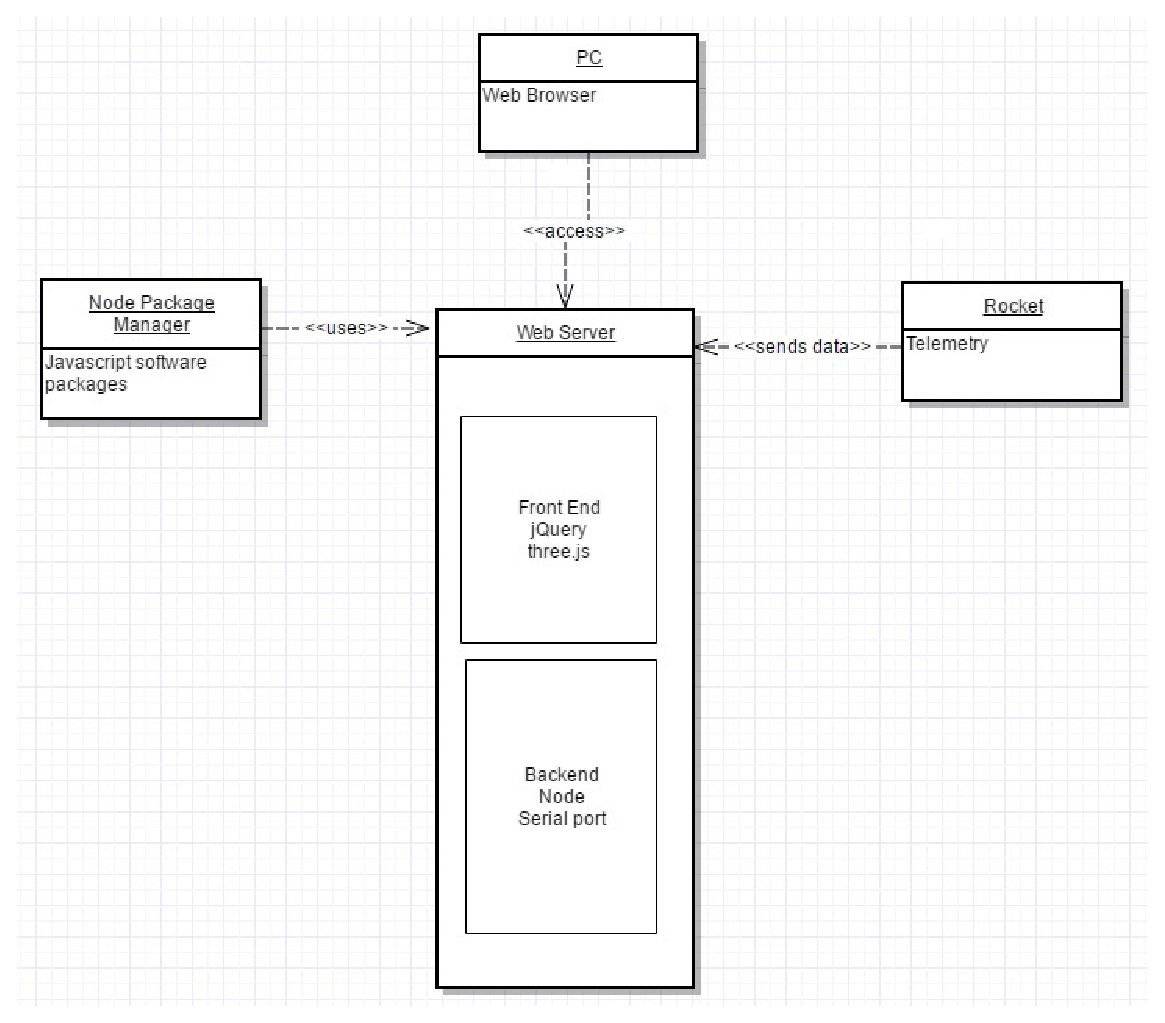
\includegraphics[width=170mm]{UMLdiagram1.eps}
		\caption{A UML diagram of what the web server is and how it is connected to everything else.}
		\label{fig:4}
	\end{figure}
	\end{center}
	\clearpage
	\index{Web browser}
	\index{Chrome}
	\index{Edge}
	\index{Firefox}
	\index{Safari}
	\newentity
	{Albert Morgan}
	{Web browser}
	{Process}
	{The web server}
	{	The client will use a web browser to connect to the Groundstation web server and access the content.
		The web browser may be any of:
		\begin{itemize}
			\item Chrome version 54 or higher
			\item Edge version 14 or higher
			\item Firefox version 49 or higher
			\item Safari version 10 or higher
		\end{itemize}
		These browsers were selected to be supported because they represent the most recent versions of the most popular web browsers in use today.
	}

	\index{Web browser}
	\index{Web server}
	\newrelationship
	{Albert Morgan}
	{Web browser / Web server}
	{Connected}
	{The web browser connects to the web server over a WiFi network via the HTTP protocol.}
	
	\newrelationship
	{Natasha Anisimova}
	{Frontend / Backend}
	{Connected}
	{The Frontend will take what the Backend of the software gives it and use 3.js to create and display information to the user.}
	
	\newrelationship
	{Terrance Lee}
	{JQuery composition}
	{Composition}
	{JQuery will be used to make our PC Controls on the website}
	
	\newrelationship
	{Natasha Anisimova}
	{3.js}
	{Part of}
	{The JavaScript Library 3.js will be used with WebGL to create the frontend of Groundstation. Figure \ref{fig:4} goes through how 3.js is a part of the creation of the frontend}
	
	\begin{center}
	\begin{figure}[htbp!]
			\centering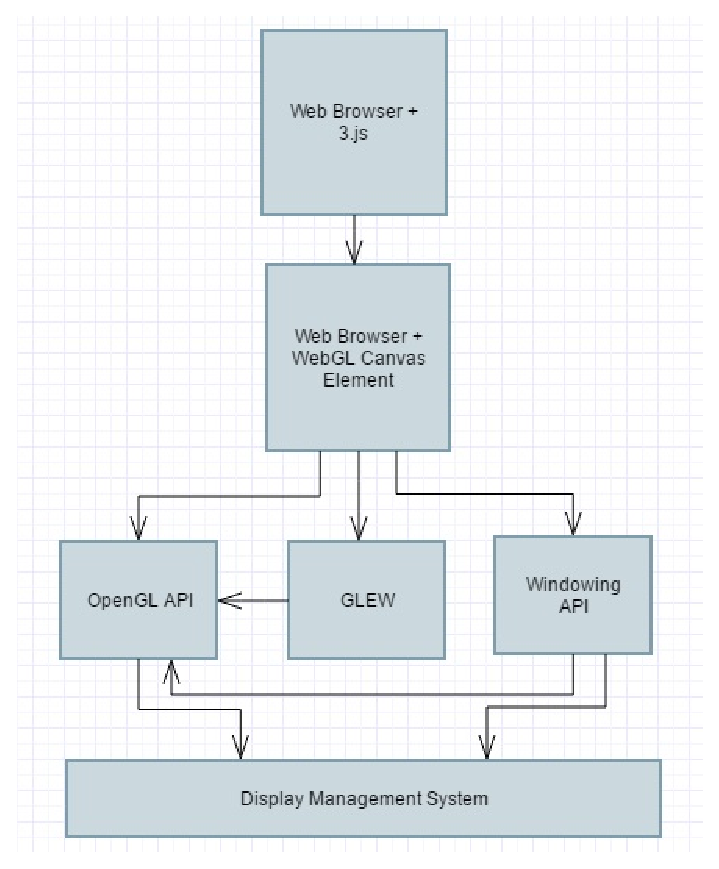
\includegraphics[width=110mm]{RelationshipDiagram.eps}
			\caption{A diagram of how 3.js is connected to WebGL and the frontend.}
			\label{fig:4}
	\end{figure}
	\end{center}
	\clearpage
	\index{Node}
	\index{Backend}
	\newrelationship
	{Albert Morgan}
	{Node / Backend}
	{Part of}
	{	Node is used by the backend to do the majority of the work.
		Node is responsible for receiving, transforming, logging, and sending the telemetry to the user.
	}
	
	\newrelationship
	{Albert Morgan}
	{Serialport use}
	{Use}
	{Node uses the serialport library to get data from the serial port.}
	
	\index{Log}
	\index{Backend}
	\newrelationship
	{Albert Morgan}
	{Log / Backend}
	{Part of}
	{
		The log is part of the backend, and will be written to by the backend and exist on the same device that runs the backend.
	}
	
	\newrelationship
	{Albert Morgan}
	{Backend / Rocket}
	{Connected}
	{The backend will retrieve data from the rocket through the serial port.
		The exact protocol used will be determined at a later date by the \ac{OSU} \ac{AIAA}
		High-Altitude Rocketry avionics team.
	}
	
	\newrelationship
	{Albert Morgan}
	{NPM / Frontend}
	{Connected}
	{NPM will be used to install all frontend software dependencies.}
	
	\index{NPM}
	\index{Backend}
	\newrelationship
	{Albert Morgan}
	{NPM / Backend}
	{Part of}
	{NPM is part of the backend, and will be used to update and install all backend software dependencies.}


	% INTERACTION SECTION
	\index{Interaction view}
	\section{Interaction View}
\newentity
	{Terrance Lee}
	{PC}
	{Component}
	{To be a tool to interact with the Raspberry Pi and the user.}
	{With the interaction of the PC and the Raspberry Pi our concern is the loss of connection due to the loss of the Wi-Fi signal.  The Raspberry Pi is just like any other Wi-Fi router and has the same issues that can drop signals.  The major issue we have to be concerned about is overheating.  We are going to be in New Mexico, out in the desert.  In Black Rock, NM we may experience temperatures up to 101 degrees.  We may be in a hotter area.  To counter this, we will have the ground station in an open area so that it can get plenty of air flow.  The second is that we will put in shade.  We will have to bring an umbrella or a tent.  This will allow the ground station to breath and stay cool.  The umbrella or tent will bring the temperature down as well.} 

	\newrelationship
	{Terrance Lee}
	{PC}
	{Component}
	{With the interaction between the website and the user we still need the PC as a tool. Our concern  in between these two is usability.  With that concern we want to make sure that everyone can understand how to navigate the website so that they do not get loss.  There are two things we want to focus on to counter this. The first thing is to use Krug’s first law of usability, the web-page should be obvious and self-explanatory.  When we make our website we need to make it so that the High-altitude Rocket team can get from point A to point B easily.   That way if they need to navigate multiple pages they won’t get lost.    The second is the “keep it simple” principle (KIS).  Doing this will help the Rocket team when they have to use anything on the page that they are on. If it is simple to use, then there is less of a chance of mistakes or misunderstandings.}
	\entityref{Rocket}
	{Structure View - Rocket}
	
	\entityref{Web Server}
	{Structure View - Web Server}
	
	\entityref{Web Browser}
	{Structure View - Web Browser}
	


	\newrelationship
	{Albert Morgan}
	{Telemetry Protocol}
	{Signal}
	{
		Once every second, the rocket will send a telemetry packet to the groundstation
		(the groundstation hardware, not the Groundstation software packagex).
		This packet will be received and transformed into a protocol that will be transmitted to the
		Groundstation software package via the serial port.
		The specification of this protocol will be determined by the avionics team at a later date.
	}

		
	\newrelationship
	{Albert Morgan}
	{JSON Protocol}
	{Signal}
	{
		Data will be stored in the log file and transmitted to the user as a list of JSON objects in the following format:\\


\noindent\{\\
\hspace*{.5cm}sensor: ...,\\
\hspace*{.5cm}value: ...,\\
\hspace*{.5cm}timestamp: ...\\
\}\\

		The JSON object has the following attributes:
		\begin{itemize}
			\item\textbf{Sensor}: This is the name of the sensor that the data is recorded from.
			This is an arbitrary string that uniquely identifies a specific sensor on the rocket.
			This string may be anything, and the user interface must understand which sensors provide which data.
			The specification of which strings correspond to which sensors will be done at a later date, after the protocol is defined.
			\item\textbf{Value}: This is the value that has been read off the sensor.
			The type of this data will depend on the specific sensor.
			\item\textbf{Timestamp}: This is the time and date that the data was received.
			This value is an integer representing the number of milliseconds that have elapsed since the epoch (January 1, 1970).
		\end{itemize}
	
			JSON objects will be transmitted to the client as a single object with a list of smaller objects inside. For example:\\

\noindent\{\\
\hspace*{.5cm}\{\\
\hspace*{1cm}sensor: altimeter,\\
\hspace*{1cm}value: 900,\\
\hspace*{1cm}timestamp: 00584747458945\\
\hspace*{.5cm}\},\\
\hspace*{.5cm}\{\\
\hspace*{1cm}sensor: tilt,\\
\hspace*{1cm}value: 4,\\
\hspace*{1cm}timestamp: 00584747458945\\
\hspace*{.5cm}\}\\
\}
}

	\index{Interface view}
	\section{Interface View}
	
	\newinterface
	{Natasha Anisimova}
	{3D View}
	{Displays the current location of the rocket.}
	{The user can interact with the view by using a mouse or track pad.}
	{
		The view will be a 3D environment that will resize as the user
		resizes the window of the web browser. If the user clicks and drags in a particular direction
		the 3D environment will move in that direction. If the user just moves the mouse without clicking, the mouse will move freely on the screen. To make orientation easier in this environment, there will be a set of buttons, shown in the figure below, that will have preset views readily available for the user. The top-most button will show a bird's eye view. The left button will show a three-fourths view facing the left side of the launch site. The right button will do the same as the left button except facing the right side of the launch site. Finally, the bottom button in this set will give a view that is directly aligned with the ground, or XZ plane, looking out into the horizon. With the help of these buttons, the user should never feel like they are unable to get back to looking at the journey of the rocket. The scroll button will zoom in and out, with the point of origin being the launch location of the rocket. Figure \ref{fig:1} shows camera view controls that will be located in the top right corner of the browser.
	}
	\begin{center}
	\begin{figure}[htbp!]
		\centering
\includegraphics[width=3.5cm]{cameracontrols.eps}
		\caption{A diagram of the camera view controls.}
		\label{fig:1}
	\end{figure}
	\end{center}


	\newinterface
	{Natasha Anisimova}
	{3D Environment}
	{Displays the current location of the rocket in the launch environment.}
	{The user can interact with the view by using a mouse or track pad.}
	{
		The 3D environment will consist of the topological map of the launch site (Spaceport America in New Mexico), with satellite images from NASA of the area mapped to it. If the user zooms past the point that the topological map covers, the ground will be displayed as a flat gray plane that goes on forever in every which way the ground would be. Since the rocket's goal is to reach 100,000 feet in height, labeling the different levels of the atmosphere that it enters would be helpful. Each level will be a transparent shade of blue, going from light to dark. Figure \ref{fig:2} shows the layers of the Earth's atmosphere.
	}
	\begin{center}
	\begin{figure}[htbp!]
		\centering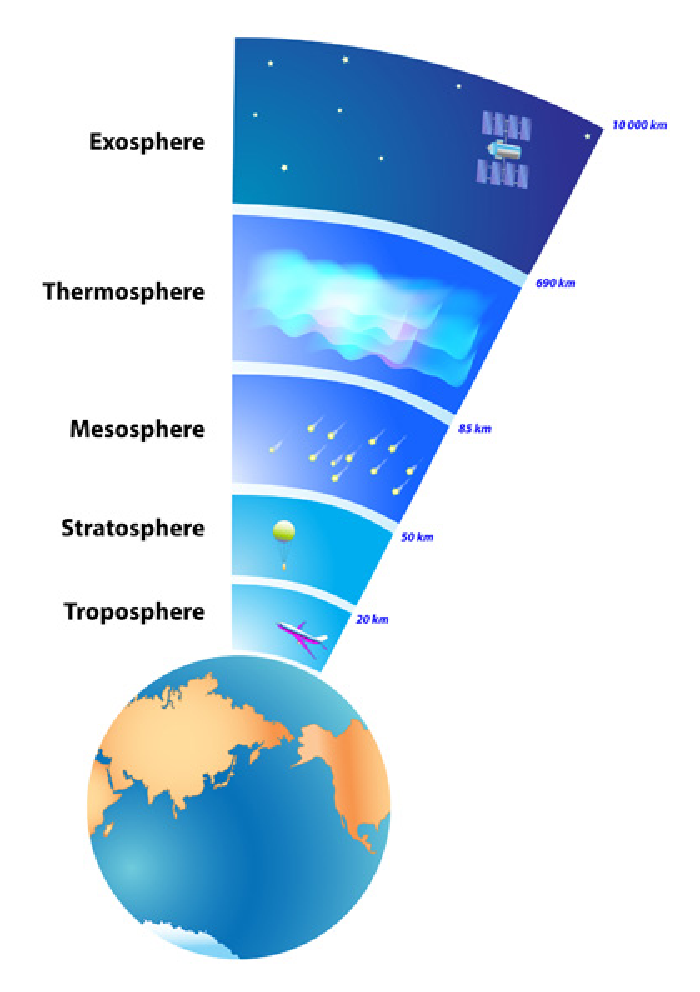
\includegraphics[width = 120mm]{earth-atmosphere-layers.eps}
		\caption{A diagram of the Earth's atmosphere.}
		\label{fig:2}
	\end{figure}
	\end{center}

%	Figure \ref{fig:2} Shows the layers of the Earth's atmosphere.
\newpage
	\newinterface
	{Natasha Anisimova}
	{Numerical Data}
	{Shows numerical data for the location of the rocket.}
	{The user can view or hide the table.}
	{
		Visual data can be hard to interpret without any numerical data to put it into perspective. Due to this, a table with the altitude, longitude, and latitude will be a part of the user interface. This table will be updated every time that a telemetry packet is received and given to the frontend of the web server.
		Figure \ref{fig:3} shows an example of how the table could be visible or hidden based off of what the user wanted.
	}
	\begin{center}
	\begin{figure}
		\centering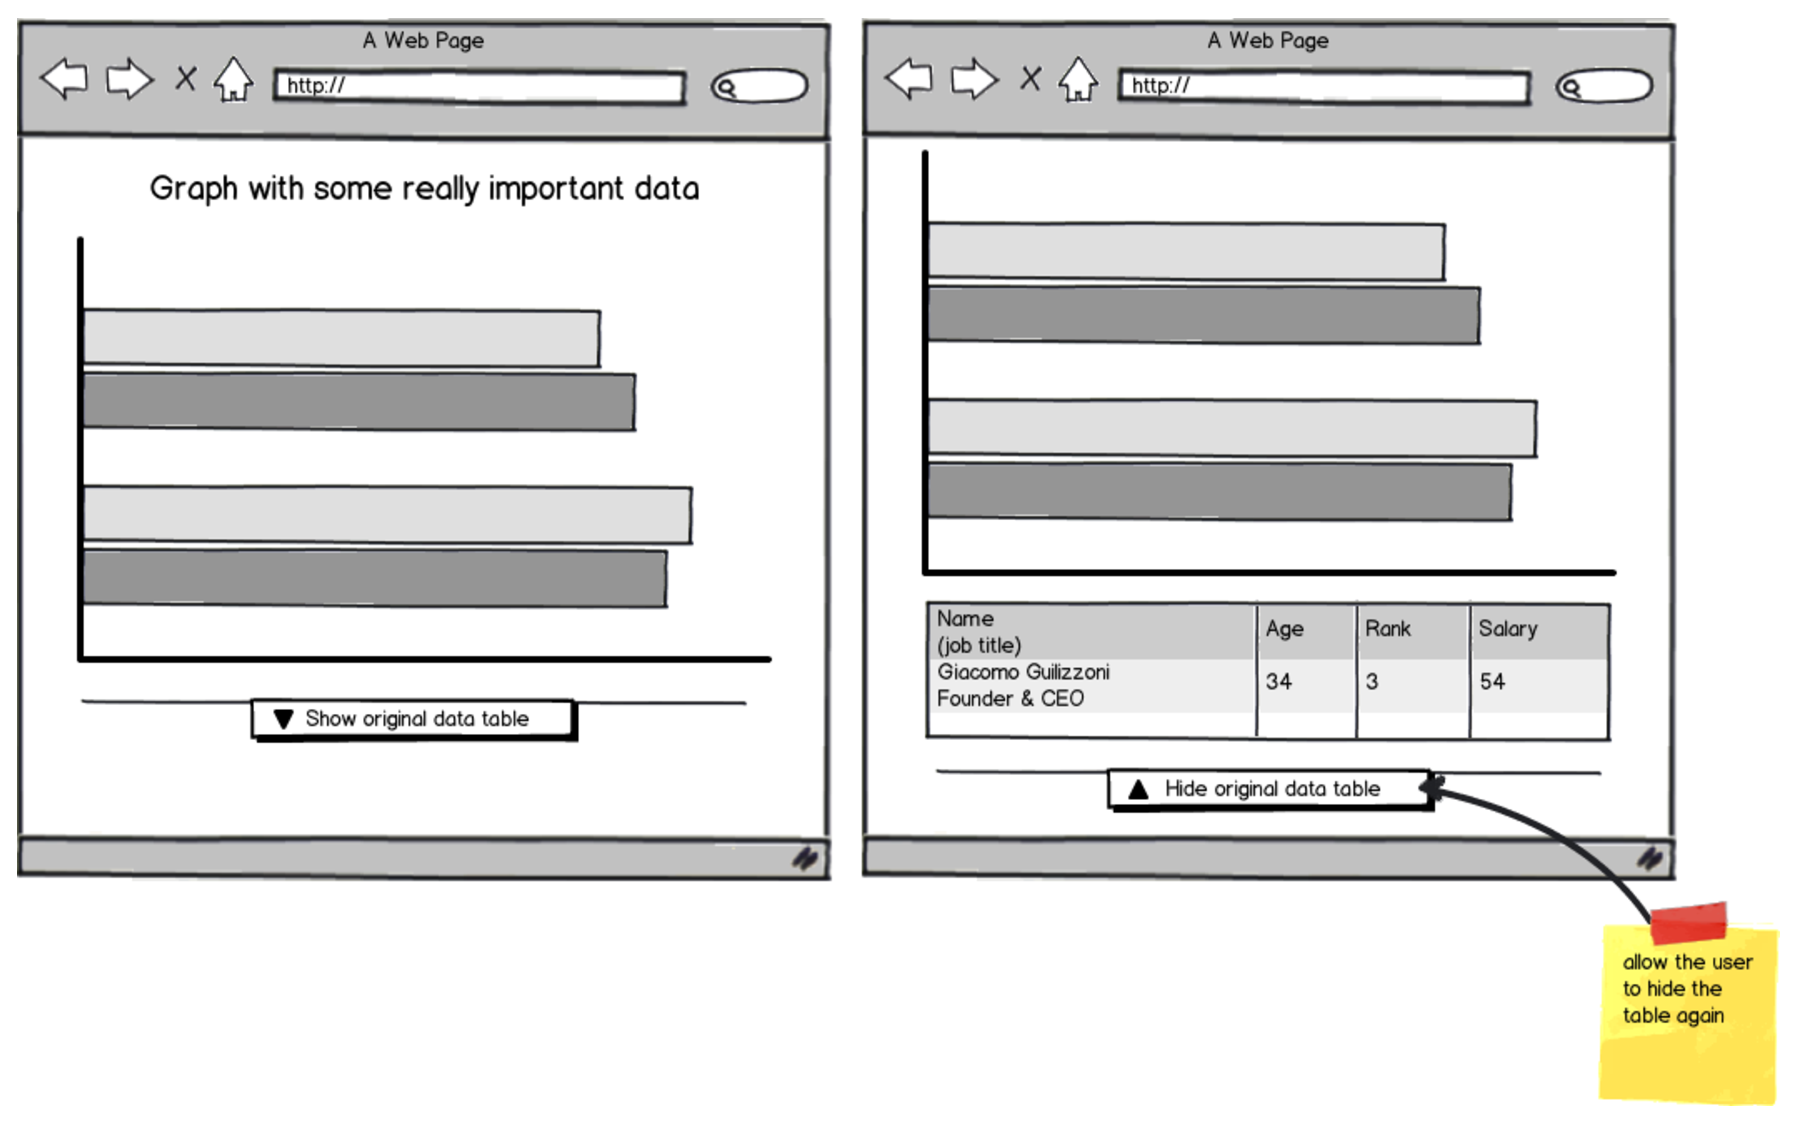
\includegraphics[width=\linewidth]{hideshowtable.eps}
		\caption{A diagram of how to show or hide a table.}
		\label{fig:3}
	\end{figure}
	\end{center}

\entityref{JQuery}
	{Structure View - JQuery}
    
\newrelationship
	{Terrance Lee}
	{JQuery interface}
	{interface}
	{ Our other concern with JQuery is the interface with the user. We want to build our dials, sliders or buttons using JQuery.  The concern is not whether or not it will work, but if it is right for the sub-teams.  We have at least five sub teams plus their members using them.  JQuery has a vast selection of PC controls. If we select the wrong setup for the team it may make it difficult for the teams to use. To counter this, we have to think about usability.  The first thing we should do is find data each team needs from the rocket.  Next find out if they are going to need PC controls. If so, then find out which ones would suit them best through user stories.  }	
	
   \index{Resource view}
	\section{Resource View}
    
     
   \newentity
	{Terrance Lee}
	{Math.Js}
	{Library}
	{Node Math library}
	{Our concern with Retrieval is loss of certain sensors.  Do to CoCom limits we lose the GPS sensor until it is under 1200 mph and under 60,000 feet. This will happen after apogee.  Also we lose accurate reading from the altimeter after 100,000 feet due to restrictions of the sensor itself.  It cannot read accurately after that height; it will just read a constant pressure until the rocket gets below that 100,000 feet. To counter act these loses we have other sensors like accelerometer and gyroscope which we can use physics and math formulas to get a location of the rocket.  With Math.js this allows us to use formulas and any other math equations to achieve this. }
     \entityref{Node}
	{Structure View - Node}
    
    \newrelationship
	{Terrance Lee}
	{Node}
	{Part of}
	{	Node is will allow us to store to the server while we are collecting the data. The data will stay on the server until we power it down.  This should allow us plenty of time to save it to our computers and hard drives.  This allows us time for resets due to software issues as well.  
		}
	
	
	\section{Revisions}


	\index{Log}
	\index{CSV}
	\newentity
	{Albert Morgan}
	{Log Revised}
	{Data store}
	{Store the data in non-volatile storage for later retrieval and update new connecting clients}
	{
		Groundstation will store telemetry in CSV.
		The log should limit the possibility of the corruption of the data due to a programming error
		and make the data easily accessible for newly connecting clients.
		Several choices were considered for the logging, including relational databases, JSON documents, CSV, and logging the raw telemetry.
		
		A relational database would be unnecessary because the data does not have any relations that need to be tracked;
		each telemetry packet is an independent piece of information.
		Logging the telemetry as it comes in from the rocket would limit the possibility of corruption.
		JSON format would make it easy to import the data into a running Node application, but may become corrupted if the program halts
		unexpectedly.
		Additionally, programming error in the JSON parsing routines could easily cause all of the data to be unusable.
		CSV format will be used for two reasons.
		First, there are no special ending characters, such as curly braces, that need to be inserted at the end of objects.
		The data will be easily readable even if the process halts unexpectedly and isn't able to finish formatting the log.
		Second, CSV files are easy to import into applications such as Microsoft Excel.
		Our teammates will be able to easily load up the data into an application of their choice for analysis after the launch.

	}


	\index{Web Server}
	\index{Raspberry Pi}
	\index{JSON}
	\index{Telemetry}
	\index{Node}
	\newentity
	{Albert Morgan}
	{Web Server Revised}
	{Part}
	{	The web server will serve three primary functions:
		\begin{itemize}
		\item Serve web pages to the clients
		\item Receive telemetry from the serial port and convert it into JSON
		\item Make the JSON data available to the clients
		\end{itemize}
	}
	{
		The web server needs to be stable so there is no data loss during the flight.
		Additionally, the web server should be as lightweight as possible to minimize the resource consumption on the Raspberry Pi.
		Groundstation will use the Node's~\cite{node} built-in web server.
		This web server was chosen over other options primarily for its stability.
		Apache uses a one-thread-per-connection model~\cite{nginx-vs-apache-our-view}, so if one thread crashes, it will not affect the rest of the connections.
		NGINX~\cite{nginx} was also considered. On large-scale servers, it is much more lightweight because it uses a many-connections-per-thread
		model.
		This allows NGINX to stay responsive even when there are thousands of connections.
		However, the number of connections will be small and the reuse of threads could reduce stability.
		For example, the thread serving the connection could crash and disconnect everyone using the software.
		Lighttpd~\cite{lighttpd} was also considered. Although Lighttpd is much more lightweight than Apache,
		it is not nearly as mature.
		Finally, we considered Node's built-in web server.
		Node's built-in web server would allow us integrate the rest of our code (which is written in Node) with the web server.
		Because we are already writing a lot of code based on the Node framework,
		writing the web server in the same language (JavaScript) will lower the time taken to develop.
		The extra time and ease of use will allow us to devote more time to testing and stability,
		effectively negating the benefit of using a more mature platform such as Apache.
		Finally, not using another piece of software for the web server will lower the time and effort it takes to install the software.
		This may be important if the software needs to be installed quickly on launch day.

		For all of the reasons listed, the built-in Node web server was selected.
	}




	\newrelationship
	{Albert Morgan}
	{JSON Protocol Revised}
	{Signal}
	{
		Data will be stored in the log file and transmitted to the user as a list of JSON objects in the following format:\\


\noindent\{\\
\hspace*{.5cm}id: ...,\\
\hspace*{.5cm}latitude: ...,\\
\hspace*{.5cm}longitude: ...,\\
\hspace*{.5cm}accelerometer\_x: ...,\\
\hspace*{.5cm}accelerometer\_y: ...,\\
\hspace*{.5cm}accelerometer\_z: ...,\\
\hspace*{.5cm}yaw: ...,\\
\hspace*{.5cm}pitch: ...,\\
\hspace*{.5cm}roll: ...,\\
\hspace*{.5cm}timestamp: ...\\
\}\\

		The JSON object has the following attributes:
		\begin{itemize}
			\item\textbf{id}: This is the id of the rocket component that the packet comes from. There are two stages to the rocket: the booster and the sustainer, and each of them will be sending packets.
The id field will inform client which part of the rocket this packet comes from, '0' for the booster, and '1' for the sustainer.
			\item\textbf{timestamp}: This is the time and date that the data was received.
			This value is an integer representing the number of seconds that have elapsed since the epoch (January 1, 1970).
			\item\textbf{other}: All other fields represent individual sensor readings. The units of these fields will be metric, except for angles, which will be encoded as degrees.
		\end{itemize}
}
	\index{Visualization}
	\index{JavaScript}
	\index{3.js}
	\index{Frontend}
	\index{WebGL}
	\newentity
{Natasha Anisimova}
{Frontend}
{Component}
{User Interface}
{
	The frontend of the web server will create and display the information that it was given by the backend. Given
	that the information has to do with location
	(longitude, latitude, and altitude), a 3D display is preferred. The
	frontend will consist of programs using 3.js and WebGL to create the visualization necessary to quickly understand the
	location of the rocket. There is a problem with the data being sent and having a 3D display. The Avonics team has
	a 3-axis gyroscope and the GPS will only be turning on at apogee. Gyroscopes tend to drift on their own so the direction
	of the rocket's flight will not be one-hundred percent accurate until the GPS. Having a simple 2D graph of the rocket's
	flight path to fall back on would be helpful in case the GPS does not turn on.
}
	

\section*{Revision History}
\vspace{0.5cm}
\begin{tabular}{l | l | l}
Name & Section Title & Date\\ \hline
Albert Morgan & Log Revised & 2017-02-15\\
Albert Morgan & Web Server Revised & 2017-02-15\\
Albert Morgan & JSON Protocol Revised & 2017-02-15\\
Natasha Anisimova & User Interface Revised & 2017-02-17\\
\end{tabular}

	%\allowdisplaybreaks
	\clearpage
	\newpage
	\section{Glossary}
		\begin{itemize}
		\index{Accuracy}
		\item \textbf{Accuracy:} The absence of errors in the telemetry GS receives, logs, and displays.
		\index{Binary data}
		\item \textbf{Binary data:} Telemetry that represents one of two states, for example, ``stage 2 activated'' and
		``stage 2 not activated.''		
		\index{COCOM limits}
		\item \textbf{COCOM limits:} The \ac{COCOM} limits apply hard limits to the speed and altitude of a GPS device.
		If a device exceeds these limits, it will stop providing GPS data.
		This is done to ensure that the device cannot be used as a missile.		
		\index{Corruption}
		\item \textbf{Corruption:} The process by which data is altered or made unreadable.
		\index{Crash}
		\item \textbf{Crash:} A software crash; the event in which a piece of software ceases operation unexpectedly.
		\index{Die}
		\item \textbf{Die:} A process dies when it ceases operation and is removed by the operating system.
		The difference between dying and crashing is that a crash may cause the program to become non-responsive,
		whereas dying causes the process to end.
		\index{Groundstation}
		\index{GS}
		\item \textbf{GS:} Groundstation, the name of our software.
		\index{Graphical display}
		\item \textbf{Graphical display:} Data that is displayed using a visualization.
		\index{Live}
		\item \textbf{Live:} Updated in real-time.
		\index{Non-volatile storage}
		\index{Storage}
		\item \textbf{Non-volatile storage:} Storage that will not be erased when the system is powered down.
		For example, a hard drive or flash storage.
		\index{Page}
		\item \textbf{Page:} A web page that users of GS may connect to in order to view the telemetry.
		\index{Process}
		\item \textbf{Process:} A running program on a computer.
		%\index{Lean angle}
		%\item \textbf{Lean angle:} The angle relative to the vertical that the rocket is currently traveling.
		\index{Raspberry Pi}
		\item \textbf{Raspberry Pi:} A small, inexpensive computing platform.		
		\index{Real-time}
		\item \textbf{Real-time:} Each telemetry datum received from the rocket must be processed and
		displayed in under one second.
		\index{Redundant sensors}
		\item \textbf{Redundant sensors:} Two or more sensors that provide the same type of data.
		\index{Reliability}
		\item \textbf{Reliability:} In the event of a software crash, the Groundstation software should automatically
		start and begin all normal functions in under five seconds.
		\index{Robustness}
		\item \textbf{Robustness:} In the event that GS receives data that is garbled or otherwise does not adhere
		to the protocol, it must continue to receive and display data and not break the real-time requirement.
		\index{Storage}
		\item \textbf{Storage:} A device where data is logged.		
		\index{Telemetry}
		\item \textbf{Telemetry:} Data received from the rocket while the rocket is in flight.
		\index{Telemetry packet}
		\index{Packet}
		\item \textbf{Telemetry packet:} The rocket will send a telemetry update once per second. Each one of these updates is a ``telemetry packet.''
		\index{Vizualation}
		\item \textbf{Visualization:} Information or data, transformed into an visual context.
		\index{X, Y, Z coordinates}
		\item \textbf{X, Y, Z coordinates:} A three coordinate system that pinpoints a point in 3D space.
		\index{XZ plane}
		\item \textbf{XZ plane:} A plane extending in the XZ directions. I.e., parallel to the ground.
	\end{itemize}
	\printindex
\bibliography{groundstation}
\bibliographystyle{IEEEtran}

\newpage
\begin{minipage}{\textwidth}	
	\SignatureAndDate{Nancy Squires}
	\SignatureAndDate{Natasha Anisimova}
	\SignatureAndDate{Terrance Lee}
	\SignatureAndDate{Albert Morgan}
\end{minipage}

\end{document}
